%Esto genérico y luego se desarrolla más sobre la aplicación
\section{Arquitectura limpia}
\label{sec:arqLimpia}
La arquitectura limpia, propuesta por Robert C. Martin \cite{martin2017clean}, se centra en la separación de responsabilidades y la creación de sistemas independientes de \textit{frameworks} de desarrollo de software y componentes externos. Esta metodología organiza el software en capas, con al menos una capa para las reglas de negocio y otra para interfaces de usuario y sistema.


El hecho de que las distintas capas sean independientes de los \textit{frameworks} permite utilizarlos como herramientas y no como estructuras rígidas. Esto evita que el sistema quede acoplado a sus restricciones. Además, es verificable ya que las reglas de negocio pueden ser evaluadas sin depender de la interfaz de usuario, la base de datos u otros elementos externos. Al ser una estructura modularizada en capas débilmente acopladas, los desarrolladores pueden validar, actualizar o reemplazar componentes individuales sin causar un impacto significativo en el resto del sistema. Esta flexibilidad reduce tiempos y costos de desarrollo. 

La independencia de la interfaz de usuario \textit{(UI por sus siglas en inglés)} es fundamental. Cambios en esta pueden realizarse fácilmente sin afectar al resto del sistema. La arquitectura limpia también garantiza independencia de la base de datos, la cual se considera un agente externo al igual que la interfaz de usuario. Es posible cambiar entre diferentes sistemas de gestión de bases de datos sin que las reglas de negocio estén atadas a una base de datos específica.

Por último, las reglas de negocio son independientes de cualquier agente externo. Esto significa que no tienen conocimiento de las interfaces hacia el mundo exterior. Esta separación permite una mayor flexibilidad y mantenimiento del sistema a lo largo del tiempo.

Los círculos en la Figura \ref{fig:cleanArch} representan diversas áreas de software. Teniendo en cuenta la figura, la regla clave para el funcionamiento de la arquitectura limpia es la regla de dependencia: \textit{``Las dependencias del código deben apuntar solo hacia adentro, hacia las políticas de más alto nivel''}\cite{martin2017clean}. En otras palabras, los círculos internos no deben conocer nada sobre los círculos externos. Específicamente, en el código interno no se debe mencionar el nombre de algo declarado en un círculo externo, ya sean funciones, clases, variables u otras entidades de software. La idea es que ningún cambio sobre los círculos externos tenga impacto sobre los círculos internos. Por otro lado, saltarse capas puede complicar la arquitectura, hacerla menos comprensible y más difícil de mantener, por lo que se recomienda no saltarse capas para mantener una estructura lo más clara y coherente posible.

\begin{figure}
    \centering
    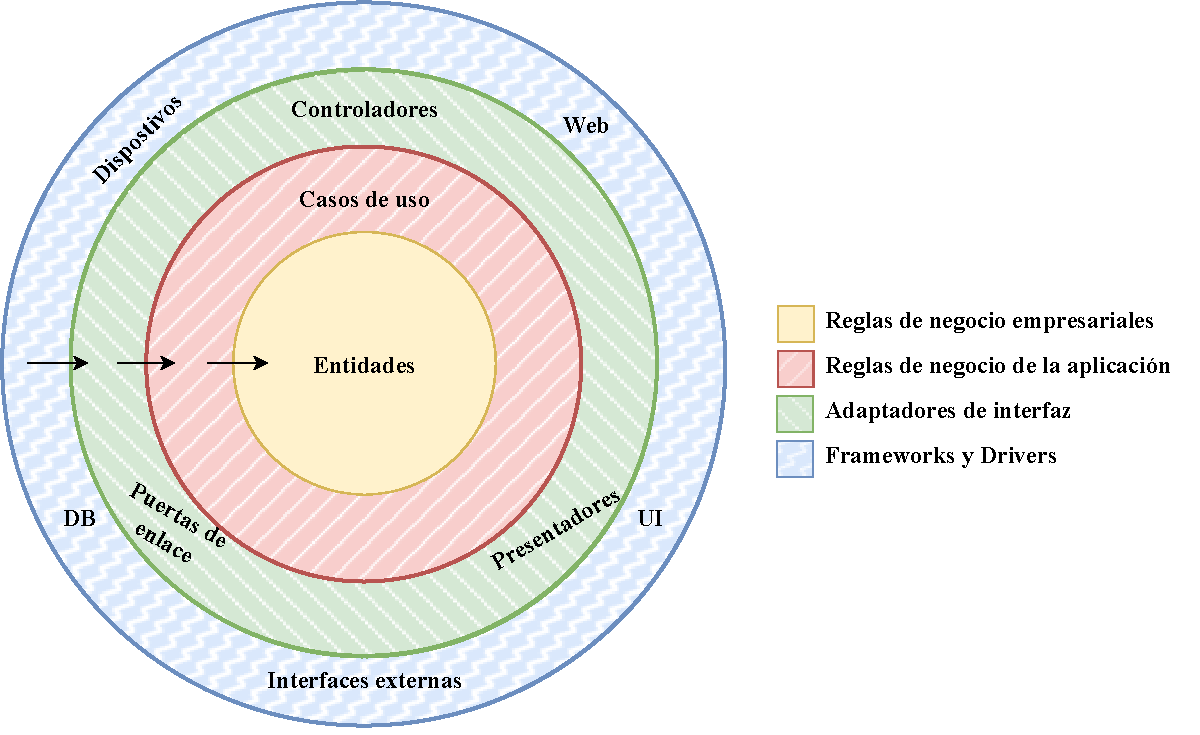
\includegraphics[width=\textwidth]{Imagenes/Arquitectura de la aplicacion movil/Arquitectura Limpia.pdf}
    \caption{Arquitectura limpia}
    \label{fig:cleanArch}
\end{figure}

Si bien la Figura \ref{fig:cleanArch} muestra cuatro círculos, no existe ninguna regla que restrinja a la utilización de estas cuatro capas siempre y cuando se aplique la regla de dependencia. Además, se debe considerar que a medida que se va hacia adentro los niveles de abstracción y políticas de alto nivel incrementan. Por otro lado, los círculos exteriores son más generales porque abordan implementaciones y detalles concretos, como las tecnologías, herramientas y componentes específicos utilizados en el sistema.

A continuación se describen las responsabilidades de cada una de las capas mostradas en la Figura \ref{fig:cleanArch}:

\begin{itemize}
    \item \textbf{Reglas de negocio empresariales: } Representan objetos de negocio fundamentales de la aplicación. Encapsulan reglas generales y de alto nivel, siendo las menos propensas a cambiar ante modificaciones externas. Una entidad puede ser un objeto con métodos, o puede ser un conjunto de estructuras de datos y funciones. Ningún cambio operativo de una aplicación específica debería afectar la capa de entidades. Por ejemplo, cambios en la interfaz de usuario de una aplicación móvil o en la seguridad no deberían afectar a estos objetos.
    \item \textbf{Reglas de negocio de aplicación: }Encapsula e implementa todos los casos de uso del sistema. Los casos de uso orquestan el flujo de datos hacia y desde las entidades, dirigiendo a dichas entidades para que utilicen sus reglas críticas de negocios y logren los objetivos del caso de uso.

    Se espera que los cambios en las reglas de negocio empresariales afecten a los casos de uso y, por lo tanto, al software de esta capa. Si los detalles en cuanto al funcionamiento relativo a un caso de uso cambian, se puede afirmar que algún código en esta capa se verá afectado.
    
    \item \textbf{Adaptadores de interfaz: }Convierten datos desde el formato más conveniente para los casos de uso y las entidades, al formato más conveniente para alguna entidad externa, y viceversa.

    \item \textbf{\textit{Frameworks} y controladores: }Generalmente está compuesta por \textit{frameworks} y herramientas como la base de datos. Es donde van todos los componentes específicos de implementación que pueden variar y ser reemplazados sin afectar la lógica central del negocio. Este tipo de componentes se mantienen en el exterior minimizando el riesgo de que cualquier cambio o problema en ellos afecte el núcleo del sistema.
\end{itemize}